\def\Ponderation{33,33}
\def\SigleNumero{STT-1920}
\def\NomCours{Méthodes statistiques}
\def\DateEvaluation{4 mars 2026}
\def\HeureEvaluation{13 h 30 à 15 h 20}
\def\Session{}
\def\NomEvaluation{Examen de reprise 1}

% Ne rien mettre entre les accolades si l'enseignant (ou l'enseignante) est aussi le coordonnateur (ou la coordonnatrice)
\def\Coordonnatrice{}
\def\Coordonnateur{}

% Ne rien mettre entre les accolades s'il y a plus d'une section
\def\Enseignant{Julien Miron}
\def\Enseignante{}

% Ne rien mettre entre les accolades s'il s'agit d'un cours à section unique
% Mettre le nom de chacun des enseignants et enseignantes entre les accolades
% Une case à cocher sera générée pour chacune des sections
\def\SectionA{}
\def\SectionB{}
\def\SectionC{}
\def\SectionD{}


\def\Directives{
\begin{enumerate}
\item Matériel autorisé:
\begin{itemize}
\item Calculatrice scientifique {\bf autorisée par la faculté des sciences et de génie};
\item Votre aide-mémoire d'une feuille recto-verso, écrit à la main.
\end{itemize}
\item Assurez-vous que cette évaluation comporte \numquestions ~exercices répartis sur \numpages{}~pages, pour un total de \numpoints{}~points.\
\item \textbf{Veuillez ne pas dégrafer votre examen.}
\item Vous devez\textbf{ justifier toutes vos réponses} par une démarche claire, sauf pour les questions à choix de réponse.\
\item Pour les questions à choix de réponse et les vrais ou faux, vous pouvez mettre un X, un crochet ($\checkmark$) ou remplir la case.\
\item Vous devez laisser tout ce qui ne servira pas durant l'examen à l'avant de la salle AVANT de rejoindre votre place.\
\item Vous n'avez droit à AUCUN appareil électronique en votre possession durant l'examen.
\item Une fois assis à votre place, vous devez demandez l'autorisation pour vous lever, même si l'examen n'est pas encore commencé.
\item Dans les 5 dernières minutes de l'examen, il sera interdit de se lever avant que TOUTES les copies n'aient été ramassées.
\end{enumerate}
\begin{itemize}
\item[$\rightarrow$] Le non-respect des consignes 7-8-9 entraînera une pénalité de 10\%.
\end{itemize}
}

\newcommand{\affichepoints}{}     % ← AVEC points
% \renewcommand{\affichepoints}{on} % ← SANS points (non vide)

\documentclass{Evaluation}
\usepackage{multicol,graphicx}

\printanswers

\begin{document}

\pageblanche

%%%%%%%%%%%%%%%% QUESTION %%%%%%%%%%%%%%%%
\begin{questions}

\question[3]\label{hist}
L'histogramme ci-dessous représente le temps d'attente (en minutes) de 50 clients choisis au hasard dans une clinique médicale. \\



\begin{center}

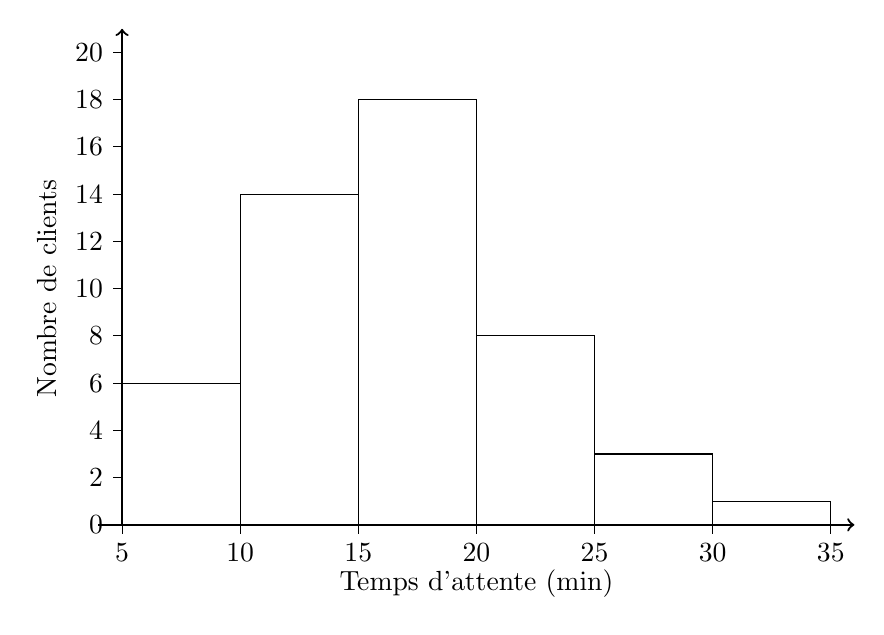
\begin{tikzpicture}[x=0.3cm,y=0.3cm]

% -------------------------------------------------
% Axes
% -------------------------------------------------
\draw[->, thick] (4,0) -- (36,0);   % axe x
\draw[->, thick] (5,0) -- (5,21); % axe y

% -------------------------------------------------
% Graduations x
% -------------------------------------------------
\foreach \x in {5,10,15,20,25,30,35}
  \draw (\x,0) -- (\x,-0.4) node[below] {\x};

% -------------------------------------------------
% Graduations y
% -------------------------------------------------
\foreach \y in {0,2,4,6,8,10,12,14,16,18,20}
  \draw (5,\y) -- (4.6,\y) node[left] {\y};

% -------------------------------------------------
% Labels
% -------------------------------------------------
\node at (20,-2.5) {Temps d'attente (min)};
\node[rotate=90] at (1.8,10) {Nombre de clients};

% -------------------------------------------------
% Histogramme (rectangles)
% Classes : [5,10[, [10,15[, [15,20[, [20,25[, [25,30[, [30,35[
% Effectifs : 6, 14, 18, 8, 3, 1
% -------------------------------------------------
\draw (5,0) rectangle (10,6);
\draw (10,0) rectangle (15,14);
\draw (15,0) rectangle (20,18);
\draw (20,0) rectangle (25,8);
\draw (25,0) rectangle (30,3);
\draw (30,0) rectangle (35,1);

\end{tikzpicture}
\end{center}


De quel type de variable s'agit-il? 
 

	
\begin{checkboxes}
        \choice Quantitative discrète
        \correctchoice Quantitative continue
        \choice Qualitative nominale
        \choice Qualitative ordinale
	\end{checkboxes}

\begin{solution}
Le temps d'attente est une mesure en minutes, donc une variable quantitative continue.
\end{solution}


\question[3] En utilisant l'histogramme de l'exercice \ref{hist}, dans quelle classe de l'histogramme se situe le quantile d'ordre 0,50 (la médiane)?

	\begin{checkboxes}
        \choice Dans la classe [5,10[
        \choice Dans la classe [10,15[
        \correctchoice Dans la classe [15,20[
        \choice Dans la classe [20,25[
        \choice Dans la classe [25,30[
	\end{checkboxes}

\begin{solution}
Le quantile 0,50 correspond à la position $0{,}50\times 50=25$. L'effectif cumulé après $[5,10[$ est $6$. Après $[10,15[$ c'est $6+14=20$. Après $[15,20[$ c'est $20+18=38$. Puisque $20<25\leq 38$, la médiane se situe dans $[15,20[$.
\end{solution}


\question[3] Quel énoncé est vrai parmi les suivants?

\begin{checkboxes}
    \choice Si $P(A)=0{,}7$ et $P(B)=0{,}4$, alors $A$ et $B$ peuvent être mutuellement exclusifs.
    \choice Si $A \cap B = \emptyset$, alors $A$ et $B$ sont indépendants.
    \correctchoice Si $A \cap B = \emptyset$, alors $P(A \cup B)=P(A)+P(B)$.
    \choice Si $A$ et $B$ sont indépendants, alors $P(A \cup B) = P(A) + P(B)$.
\end{checkboxes}

\begin{solution}
\begin{itemize}
    \item Faux: $P(A)+P(B)=1{,}1>1$, donc ils ne peuvent pas être mutuellement exclusifs.
    \item Faux: si $P(A\cap B)=0$ et $P(A),P(B)>0$, alors $P(A\cap B)\neq P(A)P(B)$, donc pas indépendants.
    \item Vrai: c'est la propriété d'additivité pour des événements mutuellement exclusifs.
    \item Faux: la formule correcte est $P(A\cup B)=P(A)+P(B)-P(A)P(B)$.
\end{itemize}
\end{solution}

\pageblanche
\question\label{couleur} Un sac contient des billes de différentes couleurs:



\begin{table}[h]
    \centering
\begin{tabular}{|c|c|}
\hline
    Couleur & Proportion\\
    \hline
     Rouge&  0,35\\
     Bleue& ?\\
     Verte& 0,05 \\
     Jaune& 0,40\\
     \hline
\end{tabular}
    \label{tab:billes}
\end{table}

Notez qu'une bille ne peut avoir qu'une seule couleur et il n'y a aucune autre couleur que les quatre mentionnées dans le tableau.


\begin{parts}

\part[6] Vous pigez une bille au hasard. Quelle est la probabilité que la bille soit bleue ou jaune?

\begin{solution}
La proportion manquante est $P(\text{Bleue})=1-0{,}35-0{,}05-0{,}40=0{,}20$. Donc $P(\text{Bleue}\cup\text{Jaune})=0{,}20+0{,}40=0{,}60$.
\end{solution}

\vspace{9cm}
\end{parts}
Pour ce qui suit, on utilise la variable aléatoire $X$, qui prend la valeur $1$ si une bille est rouge et $0$ sinon, et la variable aléatoire $Y$, qui compte le nombre de billes rouges parmi 8 billes pigées avec remise.
\begin{parts}
\setcounter{partno}{2}
\part[3] Quelle est la loi de $X$ ?
\begin{solution}
$X$ suit une loi de Bernoulli de paramètre $p=0{,}35$.
\end{solution}
\vspace{3.5cm}
\part[3] Quelle est la loi de $Y$ ?
\begin{solution}
$Y$ suit une loi binomiale $\text{Binomiale}(n=8, p=0{,}35)$.
\end{solution}
\end{parts}

\pageblanche
\question Le nombre de pannes quotidiennes dans un réseau informatique suit une loi de Poisson de paramètre $\lambda=5$.
\medskip
\begin{parts}
\part[6] Quelle est la probabilité qu'il y ait 2 pannes ou plus dans ce réseau lors d'un jour donné?

\begin{solution}
Si $N\sim\text{Poisson}(5)$, alors 
\begin{align*}
P(N\ge 2)&=1-P(N\le 1)\\
&=1-P(N=0)-P(N=1)\\
&=1-e^{-5}-5e^{-5}\\
&=1-6e^{-5}\\
&\approx 1-0{,}0404\\
&\approx 0{,}9596
\end{align*}
\end{solution}

\vspace{13cm}
\end{parts}
Un technicien inscrit chaque jour le nombre de pannes dans un fichier, durant une année.
\begin{parts}
\setcounter{partno}{1}
\part[2] On s'attend à ce que la moyenne de ces 365 observations soit environ égale à quelle valeur?

\begin{solution}
La moyenne attendue d'une observation est $\lambda=5$, donc la moyenne des 365 jours est environ $5$.
\end{solution}

\vspace{1cm}

\part[2] On s'attend à ce que la variance de ces 365 observations soit environ égale à quelle valeur?

\begin{solution}
Pour une loi de Poisson, la variance vaut $\lambda=5$. On s'attend donc à environ $5$.
\end{solution}

\end{parts}

\pageblanche
\question[3] Dans une certaine population, 60\% des individus possèdent un trait génétique donné. On sélectionne 5 individus au hasard et de façon indépendante. Soit les événements $W$:~<<Le troisième individu ne possède pas le trait>> et $Y$:~<<Exactement deux des cinq individus possèdent le trait>>. Quelles sont les probabilités associées à ces deux événements?

\begin{checkboxes}
\choice $P(W)=0{,}60$ et $P(Y)\approx 0{,}230$
\choice $P(W)=0{,}60$ et $P(Y)\approx 0{,}077$
\choice $P(W)=0{,}40$ et $P(Y)\approx 0{,}077$
\correctchoice $P(W)=0{,}40$ et $P(Y)\approx 0{,}230$
\end{checkboxes}
\vspace{0.5cm}
 


\begin{solution}
$P(W)=1-0{,}60=0{,}40$ et $P(Y)=\binom{5}{2}(0{,}60)^2(0{,}40)^3=10\times 0{,}36\times 0{,}064\approx 0{,}2304$.
\end{solution}


\question


\begin{parts}
\part[2] Si $X$ suit une loi normale
$\mathcal{N}(5, 16)$, nous avons: $P(X\leq 9)=P(Z\leq \frac{9-5}{4})=\Phi(1)$, où $Z\sim\mathcal{N}(0,1)$.

\begin{oneparcheckboxes}
    \correctchoice Vrai 
    \choice Faux
\end{oneparcheckboxes} \vspace{0.5cm}

\begin{solution}
On standardise : $Z=(X-5)/4$, donc $P(X\le 9)=P(Z\le (9-5)/4)=P(Z\le 1)=\Phi(1)$.
\end{solution}

\part[2] Si $P(A)>0$ et $P(B)>0$ et $A$ et $B$ sont mutuellement exclusifs, alors $A$ et $B$ ne sont pas indépendants.

 \begin{oneparcheckboxes}
    \correctchoice Vrai 
    \choice Faux
\end{oneparcheckboxes} \vspace{0.5cm}

\begin{solution}
Si $A \cap B = \emptyset$ alors $P(A\cap B)=0$, mais l'indépendance exigerait $P(A\cap B)=P(A)P(B)>0$. Contradiction, donc ils ne sont pas indépendants.
\end{solution}

\part[2] Si $R$ et $S$ sont deux événements indépendants, alors $P(R\cap S)=P(R)\cdot P(S)$.

 \begin{oneparcheckboxes}
    \correctchoice Vrai 
    \choice Faux
\end{oneparcheckboxes} \vspace{0.5cm}

\begin{solution}
C'est la définition même de l'indépendance de deux événements.
\end{solution}

\part[2] Le coefficient binomial $\displaystyle {M \choose j}$ nous donne le nombre de façons de choisir $j$ éléments parmi $M$.

 \begin{oneparcheckboxes}
    \correctchoice Vrai 
    \choice Faux
\end{oneparcheckboxes} \vspace{0.5cm}

\begin{solution}
Le coefficient binomial ${M \choose j}=\frac{M!}{j!(M-j)!}$ compte bien le nombre de combinaisons possibles.
\end{solution}

\part[2] Toute variable aléatoire continue dont la densité est symétrique suit nécessairement une loi normale.

 \begin{oneparcheckboxes}
    \choice Vrai 
    \correctchoice Faux
\end{oneparcheckboxes} \vspace{0.5cm}

\begin{solution}
Plusieurs lois ont une densité symétrique (ex. uniforme, Student), sans être normale.
\end{solution}

\part[2] Sur un diagramme en boîte, la longueur de la boîte représente l'étendue interquartile.

 \begin{oneparcheckboxes}
    \correctchoice Vrai 
    \choice Faux
\end{oneparcheckboxes} \vspace{0.5cm}

\begin{solution}
La boîte s'étend de $Q_1$ à $Q_3$, donc sa longueur représente $Q_3-Q_1$, soit l'étendue interquartile (IQR).
\end{solution}

\part[2] On répète 15 fois de façon indépendante une épreuve de Bernoulli dont la probabilité de succès est de 0,30. Alors le nombre d'échecs suit une loi $\text{Binomiale}(n = 15, p = 0{,}70)$.

 \begin{oneparcheckboxes}
    \correctchoice Vrai 
    \choice Faux
\end{oneparcheckboxes} \vspace{0.5cm}

\begin{solution}
Le nombre de succès suit $\text{Binomiale}(15, 0{,}30)$ et le nombre d'échecs suit $\text{Binomiale}(15, 0{,}70)$.
\end{solution}

\end{parts}

\newpage
\question On suppose que le taux de cholestérol (en mg/dL) suit une loi normale de moyenne 200 et de variance $10^2$. On utilisera $X$ pour dénoter cette variable aléatoire. Donc $X\sim\mathcal{N}(200, 10^2)$.

\begin{parts}
\part[3] Quelle est la probabilité qu'un individu choisi au hasard ait un taux de cholestérol inférieur ou égal à 200? Justifiez votre réponse!

\begin{solution}
Par symétrie de la loi normale autour de la moyenne, $P(X\le 200)=0{,}5$.
\end{solution}

\vspace{3cm}

\part[8] Nous aimerions connaître la probabilité qu'un individu choisi au hasard ait un taux de cholestérol inférieur à 185 ou supérieur à 215. Calculez cette probabilité en utilisant la table de la loi normale. Utilisez 4 chiffres après la virgule dans vos calculs et dans votre réponse.  
\begin{solution}
$z_1=\frac{185-200}{10}=-1{,}5$ et $z_2=\frac{215-200}{10}=1{,}5$. Par symétrie:
$$P(X<185)+P(X>215)=\Phi(-1{,}5)+[1-\Phi(1{,}5)]=2\times\Phi(-1{,}5)=2\times 0{,}0668=0{,}1336.$$
\end{solution}

\vspace{13cm}

\part[4] Si on prenait un échantillon de 25 personnes, quelle serait la variance de la moyenne échantillonnale $\overline{X}$? Donnez la valeur de cette variance!  

\begin{solution}
$\mathrm{Var}(\overline{X})=\sigma^2/n=100/25=4$.
\end{solution}

\end{parts}

\pageblanche

\question Une association agricole évalue qu'une brebis adulte coûte en moyenne 80\$ par année à nourrir, avec un écart-type de 12\$. Voici les diagrammes de la fonction de densité et de la fonction de répartition du modèle probabiliste supposé.

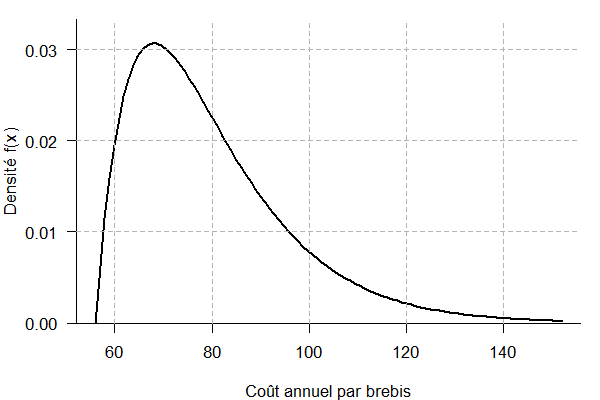
\includegraphics[width=8cm]{chi-den.png}
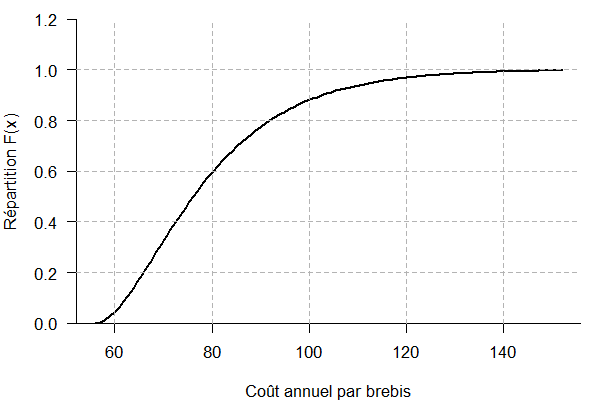
\includegraphics[width=8cm]{chi-rep.png}

\begin{parts}
\part[2] En utilisant les diagrammes, quelle est la probabilité approximative que le coût annuel par brebis soit supérieur à 80\$?

\begin{solution}
D'après la fonction de répartition, $F(80)\approx 0{,}6$, donc $P(X>80)\approx 1-0{,}6=0{,}4$.
\end{solution}

\vspace{2cm}

\part[2] En utilisant les diagrammes, dites si la loi normale convient pour modéliser cette variable aléatoire. Donnez au moins une raison!

\begin{solution}
Non, la densité n'est pas symétrique (asymétrie à droite), ce qui va à l'encontre d'une loi normale.
\end{solution}

\vspace{1.5cm}

\part[8] Une ferme possède un élevage de 225 brebis. Donnez une approximation de la probabilité que le montant annuel à débourser pour les nourrir dépasse 18\ 180\$.

\newpage

\begin{solution}
Par le TCL, la somme $S=\sum_{i=1}^{225}X_i$ est approximativement normale avec $E(S)=225\times 80=18\,000$ et $\sigma_S=12\sqrt{225}=180$. Ainsi:
$$P(S>18\,180)\approx 1-\Phi\!\left(\frac{18\,180-18\,000}{180}\right)=1-\Phi(1)\approx 1-0{,}8413=0{,}1587.$$
\end{solution}


\end{parts}

\question[5] Soit $A$ et $B$, deux événements pour lesquels $P(A\cap B)=0{,}15$, $P(A\cap \bar{B})=0{,}25$ et $P(B\cap \bar{A})=0{,}20$.

Que vaut $P(A\cup B)$?

\begin{solution}
$P(A\cup B)=P(A\cap B)+P(A\cap \bar{B})+P(B\cap \bar{A})=0{,}15+0{,}25+0{,}20=0{,}60$.
\end{solution}

\pageblanche
%
\includepdf[pages={1}]{Tables_lois.pdf}

\end{questions}
\end{document} 
